\subsection{Lewis Structure}
\begin{minipage}{0.49\linewidth}
 \textbf{Drawing Lewis Structures}\\
1. Sum VE of all atoms\\
2. Write symbols and connect with single bonds\\
3. Complete octets around non-central atoms\\
4. Place remaining VE around central atom\\
5. Try multiple bonds if central atom does not have octet\\
\vspace{3pt}\\
\textbf{Alternative Lewis Structure}\\
$\circ$ More than one Lewis Structure possible\\
$\circ$ Calculate formal charges of each atom\\
$\circ$ Formal charges closest to zero with negative formal charges on more EN atoms is dominant\\
$\circ$ A molecule is most stable when it has the least overall formal charge\\
\fbox{Formal Charge $=$ Atom's VE $- \frac{1}{2}$ (Atom's bonding e's) $-$ (Atom's non-bonding e's)}
\end{minipage}
\begin{minipage}{0.24\linewidth}
      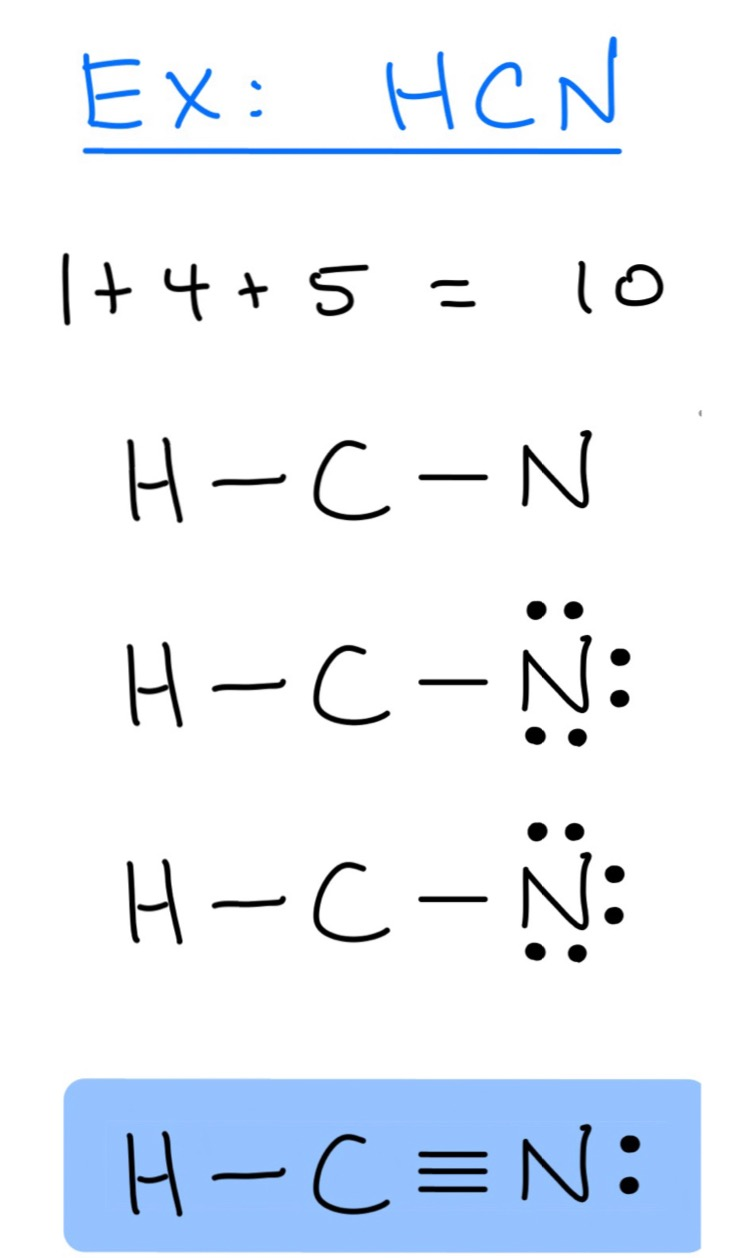
\includegraphics[width = 0.6\linewidth]{images/Lewis_Structure_HCN.jpeg}
      \\
      \\
\end{minipage}
\begin{minipage}{0.24\linewidth}
    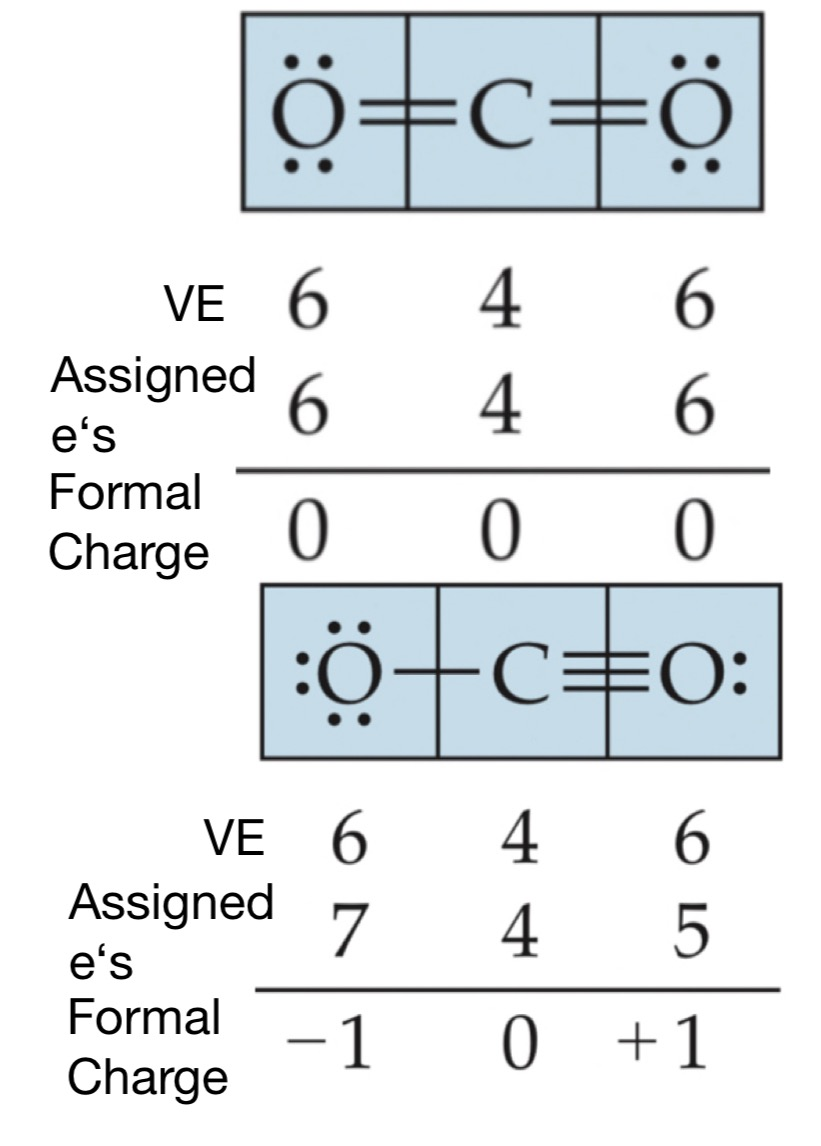
\includegraphics[width = \linewidth]{images/Lewis_Structure_CO2.jpeg}
\end{minipage}

